\documentclass{beamer}
\mode<presentation>
{
	\usetheme{Madrid}

    \definecolor{unisinos}{RGB}{67,40,117}
    \usecolortheme[named=unisinos]{structure}

	\usefonttheme{professionalfonts}
    \usebackgroundtemplate{
\includegraphics[width=\paperwidth,height=0.978\paperheight]{template_unisinos}}

 	\beamertemplatenavigationsymbolsempty
 	\setbeamertemplate{footline}
	{
	  \leavevmode%
	  \hbox{%
	  \begin{beamercolorbox}[wd=.12\paperwidth,ht=2.25ex,dp=1ex,center]{author in head/foot}%
	    \usebeamerfont{author in head/foot}\insertshortauthor
	  \end{beamercolorbox}%
	  \begin{beamercolorbox}[wd=.88\paperwidth,ht=2.25ex,dp=1ex,center]{title in head/foot}%
	    \usebeamerfont{title in head/foot}\insertshorttitle\hspace*{3em}
	    \insertframenumber{} / \inserttotalframenumber\hspace*{1ex}
	  \end{beamercolorbox}}%
	  \vskip0pt%
	}
 	\setbeamertemplate{caption}[numbered]
 	\usepackage{caption}

 	\usepackage[brazil]{babel}		% Idioma do documento
	\usepackage{siunitx}
	\usepackage{ragged2e}
	\usepackage{float}
    \usepackage{indentfirst} }
    \usepackage[alf]{abntex2cite}		% Citações padrão ABNT
	\usepackage{color}			% Controle das cores
	\usepackage[T1]{fontenc}		% Selecao de codigos de fonte.
	\usepackage{graphicx}			% Inclusão de gráficos
	\usepackage[utf8]{inputenc}		% Codificacao do documento (conversão automática dos acentos)
	\usepackage{txfonts}			% Fontes virtuais

\title[Seminário I - Estudo sobre arquiteturas de conversores AD]{Seminário I - Estudo sobre arquiteturas de conversores AD}
\author[Piaia, G. A.]{
	{\fontsize{10}{8}\selectfont \textbf{Aluno:} Guilherme Angelo Piaia} \\
	{\fontsize{10}{8}\selectfont \textbf{Professor}: Cesar Crovato}
}
%\institute[UNISINOS]{UNISINOS - Universidade do Vale do Rio dos Sinos \\ Engenharia de Controle e Automação}

\date{\today}

\begin{document}

%%%%%%%%%%%%%%%%%%%%%%%%%%%%%%%%%%%

\begin{frame}
	\begin{minipage}{1\linewidth}
		\centering
		    \textbf{UNISINOS - Universidade do Vale do Rio dos Sinos} \\ Mestrado Profissional em Engenharia Elétrica
	\end{minipage}
	\titlepage
\end{frame}

%%%%%%%%%%%%%%%%%%%%%%%%%%%%%%%%%%%

\begin{frame}{Sumário}
	\tableofcontents[]
\end{frame}

%%%%%%%%%%%%%%%%%%%%%%%%%%%%%%%%%%%

\section{Introdução}
\begin{frame}{Introdução}
	\begin{columns}
	    \begin{column}{0.50\textwidth}
			\begin{itemize}
				\justifying
				\item Este trabalho contem um breve compilado sobre topologias de ADCs (\textit{Analog to digital converters}):
				\begin{itemize}
					\justifying
					\item SAR (\textit{successive approximation register})
					\item SigmaDelta ($\Sigma - \delta$)
		 			\item Flash
					\item Pipeline
					\item Dual Slope
		    	\end{itemize}
		    \end{itemize}
	    \end{column}

	    \begin{column}{0.5\textwidth}
			\begin{figure}[H]
			    \centering
			    \begin{center}
			    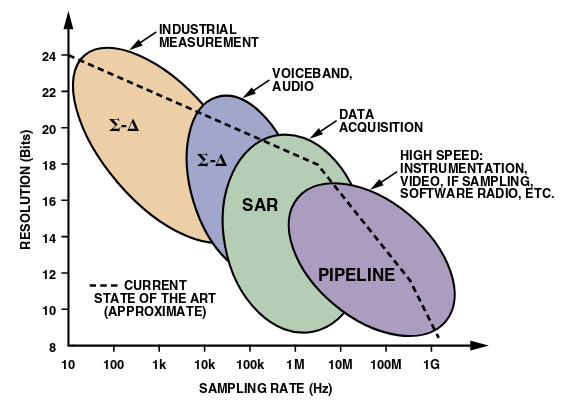
\includegraphics[width=\textwidth]{img/adcs}
			  \caption{Relações entre as principais arquiteturas de conversores AD (2005).}
			    \label{fig:sar}
			  \end{center}
			\end{figure}
	    \end{column}
	\end{columns}
\end{frame}

%%%%%%%%%%%%%%%%%%%%%%%%%%%%%%%%%%%

\section{SAR}

\begin{frame}{SAR}
\begin{columns}
    \begin{column}{0.50\textwidth}
		\begin{itemize}
			\item Utilizado para aquisição de dados;
			\item É a arquitetura mais comum, principalmente se o projeto necessita de várias entradas e multiplexadas;
			\item Possuem elevada performance, atingindo amostragens na casa de 3MSPS;
			\item Interfaceado via SPI ou I2C;
			\item \textit{sample-and-hold}(SHA) mantém constante o sinal durante a conversão;
		\end{itemize}
    \end{column}

    \begin{column}{0.5\textwidth}
		\begin{figure}[H]
		    \centering
		    \begin{center}
		    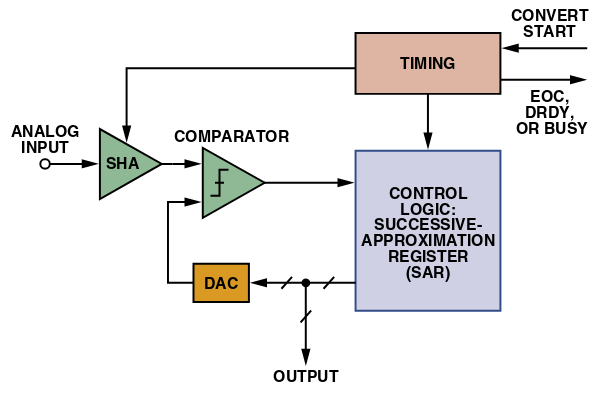
\includegraphics[width=\textwidth]{img/sar}
		  \caption{Diagrama da arquitetura SAR.}
		    \label{fig:sar}
		  \end{center}
		\end{figure}
    \end{column}
\end{columns}
\end{frame}

%%%%%%%%%%%%%%%%%%%%%%%%%%%%%%%%%%%

\begin{frame}{SAR}
	\begin{itemize}
		\item A conversão começa quando o DAC é configurado para a metade da escala;
		\item O comparador determina se o sinal de entrada é maior ou menos que o do DAC, salvando em um registrador o bit mais significativo (MSB);
		\item Após isso, o DAC é configurado para $\frac{1}{4}$ ou $\frac{3}{4}$, dependendo do resultado da operação anterior;
		\item Após a conversão, o sinal de \textit{BUSY} é atualizado;
	\end{itemize}
\end{frame}

%%%%%%%%%%%%%%%%%%%%%%%%%%%%%%%%%%%

\section{$\Sigma - \delta$}

\begin{frame}{$\Sigma - \delta$}
\begin{columns}
    \begin{column}{0.50\textwidth}
		\begin{itemize}
			\item Utilizado para instrumentação que exigem elevada resolução (16 - 24 bits);
			\item Opera na numa faixa de centenas de Hertz;
			\item Como apresenta \textit{oversampling},  simplifica o filtro de \textit{antialiasing};
			\item Alta resolução;
			\item Lento pelo processo de \textit{oversampling};
		\end{itemize}
    \end{column}

    \begin{column}{0.5\textwidth}
		\begin{figure}[H]
		    \centering
		    \begin{center}
		    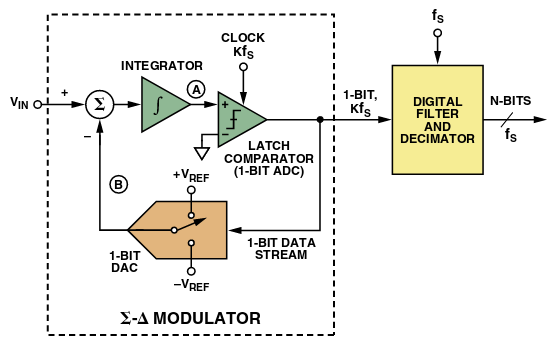
\includegraphics[width=\textwidth]{img/sigma}
		  \caption{Diagrama da arquitetura $\Sigma - \delta$ de primeira ordem.}
		    \label{fig:sar}
		  \end{center}
		\end{figure}
    \end{column}
\end{columns}
\end{frame}


%%%%%%%%%%%%%%%%%%%%%%%%%%%%%%%%%%%

\section{Flash}

\begin{frame}{Flash}
\begin{columns}
    \begin{column}{0.50\textwidth}
		\begin{itemize}
			\item A conversão ocorre em um único ciclo de clock;
			\item Ocupam grande área e são de elevada potência;
			\item O tempo de conversão é a soma dos delays com o delay lógico;
			\item Baixa resolução;
		\end{itemize}
    \end{column}

    \begin{column}{0.5\textwidth}
		\begin{figure}[H]
		    \centering
		    \begin{center}
		    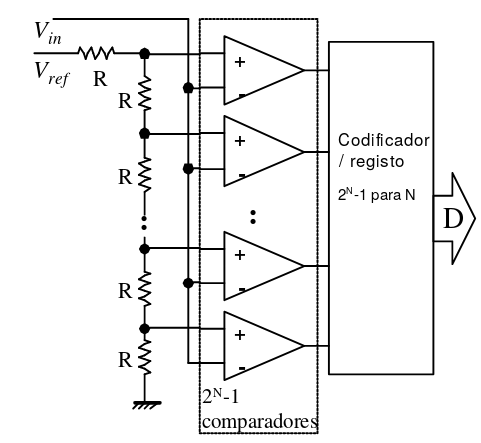
\includegraphics[width=\textwidth]{img/flash}
		  \caption{Diagrama da arquitetura Flash.}
		    \label{fig:sar}
		  \end{center}
		\end{figure}
    \end{column}
\end{columns}
\end{frame}

%%%%%%%%%%%%%%%%%%%%%%%%%%%%%%%%%%%

\section{Pipeline}

\begin{frame}{Pipeline}
\begin{columns}
    \begin{column}{0.50\textwidth}
		\begin{itemize}
			\item Utilizado em aplicações que requerem amostragens maiores que 5 MSPS;
			\item Topologia semelhante a SAR;
			\item Utilizado em analizadores de espectro, radares e Rádio via Software;
			\item Baixa resolução (6-8 bits);
		\end{itemize}
    \end{column}

    \begin{column}{0.5\textwidth}
		\begin{figure}[H]
		    \centering
		    \begin{center}
		    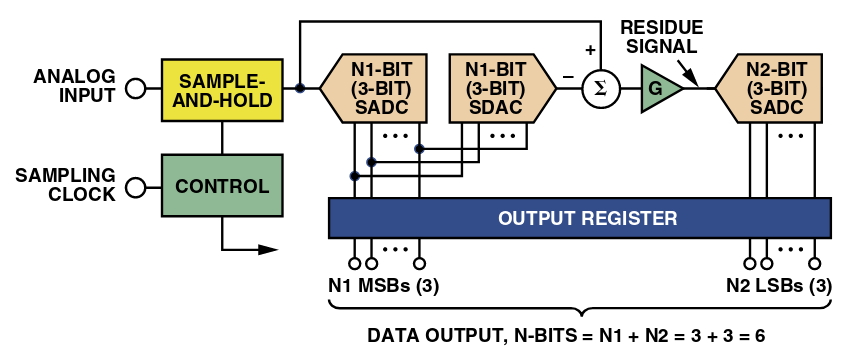
\includegraphics[width=\textwidth]{img/pipeline}
		  \caption{Diagrama da arquitetura Pipeline de primeira ordem.}
		    \label{fig:sar}
		  \end{center}
		\end{figure}
    \end{column}
\end{columns}

\end{frame}

%%%%%%%%%%%%%%%%%%%%%%%%%%%%%%%%%%%

\section{Dual Slope}

\begin{frame}{Dual Slope}
\begin{columns}
    \begin{column}{0.50\textwidth}
		\begin{itemize}
			\item Utiliza relés e integradores;
			\item O ruido na entrada é reduzido pela média;
			\item O valor do capacitor e clock não afetam a acurácia;
			\item Boa linearidade;
			\item Aplicável em instrumentação com necessidade de alta resolução;
			\item Baixa amosatragem, na casa de 10 SPS;
			\item É usado em voltímetros digitais;
		\end{itemize}
    \end{column}

    \begin{column}{0.5\textwidth}
		\begin{figure}[H]
		    \centering
		    \begin{center}
		    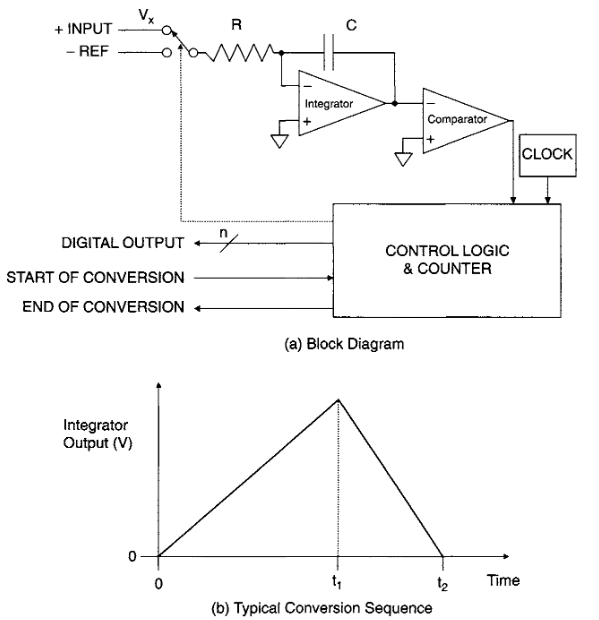
\includegraphics[width=0.85\textwidth]{img/dual-slope}
		  \caption{Diagrama da arquitetura Dual-Slope.}
		    \label{fig:sar}
		  \end{center}
		\end{figure}
    \end{column}
\end{columns}
\end{frame}

%%%%%%%%%%%%%%%%%%%%%%%%%%%%%%%%%%%

\section{Referências Bibliográficas}
\begin{frame}{Referências Bibliográficas}
	[1] Kester, W., “Which ADC Architecture Is Right for Your Application?”, Analog Dialogue 39-06, Junho de 2005.

    [2] Austerlitz, H., "Data Acquisition Techniques Using PCs", Second Edition, 2003.
\end{frame}


%%%%%%%%%%%%%%%%%%%%%%%%%%%%%%%%%%%

\begin{frame}{Agradecimentos}
		\begin{center}
			{\Huge Obrigado pela Atenção!}
		\end{center}
\end{frame}

\end{document}
